% Chapter 3

\chapter{Theories and Tools Used}
This chapter will cover some theories and tools used in the various machine learning algorithms and our analysis.
\setlength{\belowdisplayskip}{1pt} \setlength{\belowdisplayshortskip}{1pt}
\setlength{\abovedisplayskip}{1pt} \setlength{\abovedisplayshortskip}{1pt}

\section{Expectation Maximisation (EM) Algorithm} \label{2.1}
EM is an iterative method that attempts to find the maximum likelihood estimator of a parameter $\theta$ of a parametric probability distribution \cite{Gupta}. As a general procedure, EM is used to estimate parameters for probabilistic models with hidden or latent variables. EM algorithm is used both in Gaussian Mixture Model (refer to Chapter \ref{3.2}) and K-means (will not be covered in this report). 
\subsection{Outline}
Consider a probabilistic model in which we have: observed data $y$, a parametric density $p(y|\theta)$, a description of some complete data $x$ that we wish we had, and the parametric density $p(x|\theta)$. We assume that the complete data can be modelled as a continuous random vector $X$ with density $p(x|\theta)$, where $\theta \in \omega$ for some set $\omega$. We do not observe $X$ directly; instead, we observe a realization $y$ of the random vector $Y$ that depends on $X$. 

Given that we only have $y$, we want to find the maximum likelihood estimate (MLE) of $\theta$:
\begin{equation*}
\theta_{\text{MLE}} = \operatorname{arg\,max}_{\theta \in \omega} \log p(y|\theta)
\end{equation*}
However, for some problem it is difficult to solve the above optimization problem and here where EM comes to help. We make a guess about the complete data $X$ and solve for the $\theta$ that maximizes the (expected) log-likelihood of $X$. And once we have an estimate for $\theta$, we can make a better guess about the complete data $X$, and iterate. Here are the steps in summary:
\begin{itemize}
	\item Let $m=0$ and make an initial estimate $\theta^{(m)}=\theta$.
	\item Given the observed data $y$ and pretending for the moment that our current guess $\theta^{(m)}$ is correct, formulate the conditional probability distribution $p(x|y, \theta^{(m)})$ for the complete data $x$.
	\item Using the conditional probability distribution $p(x|y, \theta^{(m)})$ calculated in Step 2, form the \textit{conditional expected log-likelihood}, which is called the $Q$-function:
	\begin{equation*}
	Q(\theta|\theta^{(m)}) = \int_{\omega (y)} \log p(x|\theta)p(x|y, \theta^{(m)})dx = \mathbb{E}_{X|y,\theta^{(m)}} \log p(X|\theta)
	\end{equation*}
	\item Find the $\theta$ that maximizes the $Q$-function; the result is our new estimate $\theta^{(m+1)}$.
	\item Let $m:=m+1$ and go back to Step 2. The EM algorithm does not specify stopping criterion; standard criterion is to iterate until the estimate stops changing: $||\theta^{(m+1)}-\theta^{(m)}|| < \epsilon$ for some $\epsilon>0$, or to iterate until the log-likelihood $l(\theta) = \log p(y|\theta)$ stops changing: $|l(\theta^{(m+1)})-l(\theta^{(m)})|<\epsilon$ for some $\epsilon>0$.
\end{itemize}

The monotonicity of the EM algorithm guarantees that as EM iterates, its guesses will not get worse in terms of their likelihood (the proof can be referred to \cite{Bishop2013}), but the monotonicity alone cannot guarantee the convergence of the sequence $\{\theta^{(m)}\}$. Hence, in practice, we perform EM algorithm multiple times to get the best fit. 
%----------------------------------------------------------------------------------------

\section{Determining Optimal Number of Clusters} \label{2.2}
Here we describe a method to determine the optimal number of clusters for Gaussian Mixture Model.
\subsection{BIC and AIC} \label{2.2.1}
%Akaike, H.: A new look at the statistical model identification
%Schwarz, G.: Estimating the dimension of a model
%GMM for Time Series Modelling, Forecasting and Interpolation
When we want to find optimal number of clusters from various clustering algorithms, too few components are not able to model the distribution appropriately, while having too many components cause issues of overfitting. The number of components can be selected according to Akaike Information Criterion (AIC) \cite{Akaike1998} or the Bayesian Information Criterion (BIC) \cite{Schwarz1978}. 
\subsubsection{Outline}
BIC and AIC impose a penalty on the total number of parameters, scaled by the logarithm of sample size, so as to strike a balance between the goodness-of-fit and the model complexity.
Both are expressed as a function of the log-likelihood of the converged mixture model:
\begin{align*}
AIC  &= -2\log L(\theta) + 2P\\
BIC &= -2\log L(\theta) + \log(N)P
\end{align*}
where $P$ is the number of free parameters and $N$ is the number of data points. The clustering algorithm (Mixture Model in our case) is run for several different values of $K$, and the model which minimises the chosen criterion is selected. As $\log(N)>2$ in most cases, BIC more aggresively penalises an increase in $P$, generally resulting in a smaller choice for $K$ than by AIC. Lower AIC or BIC values indicates better fitting models. We should also ensure that our choices for $k$ and the covariance matrix structure is appropriate for our application. 

\subsection{Elbow Method Analysis} \label{2.2.2}
For \textit{k-means}, since we do not know the definitive answer on the optimal number of clusters, we need a method to quantify the quality of clustering. \textit{Elbow Method} is a graphical tool that helps us to estimate the optimal number of cluster $k$ for our task. 
\subsubsection{Outline}
The elbow method plots the value of the cost function produced by different values of $k$. This is motivated by the use of intrinsic metrics - such as the within-cluster sum-of-squared-error (distortion). Intuitively, we can say that, if $k$ increases, the distortion will decrease; each cluster will have fewer constituent instances, and the instances will be closer to their respective centroids. However, the improvements to the average distortion will decline as $k$ increases. The value of $k$ at which the improvement to the distortion declines the most is called the elbow (Figure \ref{fig: elbow}). Here is the method in summary:
\begin{itemize}
	\item Find the sum of intra-cluster distances between points $\in D_k$ in a given cluster $C_k$, \\$C_k=\sum\limits_{x_i \in D_k}\sum\limits_{x_j \in D_k} \lVert x_i-x_j \rVert ^2 = 2n_k \sum\limits_{x_i \in D_k} = \lVert x_i - \mu _k \rVert ^2$
	\item Find the normalized intra-cluster sums of squares: measure compactness of our clustering, $W_k = \sum\limits_{k=1}^K \frac{1}{2n_k}C_k$
	\item Look at the $\%$ of variance explained as a function of the number of clusters
\end{itemize}

\begin{figure}[h] 
	\centering
	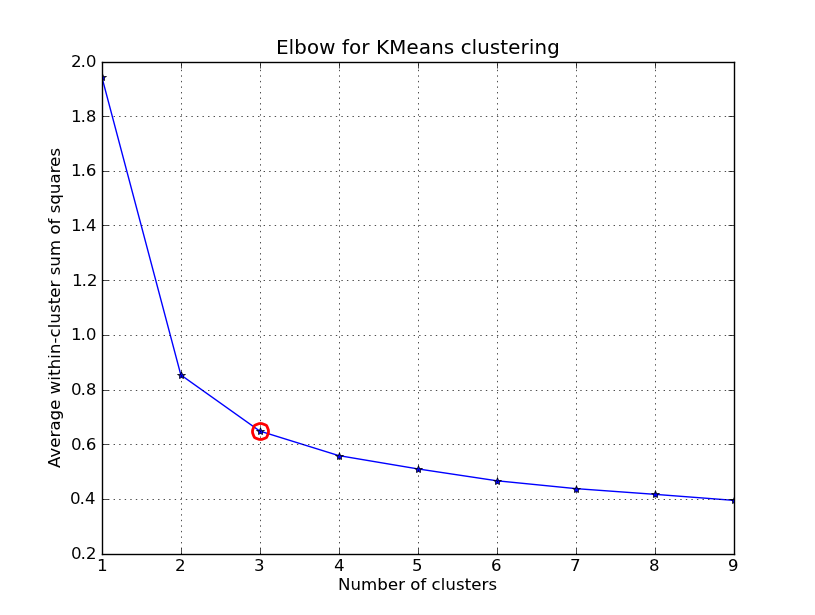
\includegraphics[scale= 0.5]{Figures/elbow_curve_expected.png}
	\caption{Ideal elbow curve where it easy to identify the 'elbow' (red circle)}
	\label{fig: elbow}
\end{figure}

\subsection{Gap Statistic} \label{2.2.3}
Gap Statistic \cite{Tibshirani2001} is another popular method used to determine the optimal number of clusters from various clustering algorithms such as \textit{k-means}. 
\subsubsection{Outline}
Given our data $\{x_{ij}\}, i =1,2,\dots,n, j = 1,2,\dots, p$, consist of $p$ features measured on $n$ independent observations. Let $d_{ii'}$ denote the distance between observations $i$ and $i'$. For simplicity, we use euclidean distance $d_{ii'} = \sum_j (x_{ij}-x_{i'j})^2$.
Suppose that we have clustered the data into $k$ clusters $C_1, C_2, \dots, C_k$, with $C_r$ denoting the indices of observations in cluster $r$, and $n_r = |C_r|$. Let $D_k$ and $W_k$ be the same as that in elbow curve analysis. Then, the idea of gap statistic analysis is to standardize the graph of $\log(W_k)$ by comparing it with its expectation under an appropriate null reference distribution of the data. Our estimate of the optimal number of clusters is the the value of $k$ for which $\log(W_k)$ falls the farthest below this reference curve. Hence, we define $Gap_n(k) = E_n^*\{\log W_k\}-\log W_k$ where $E_n^*$ denotes the expectation under a sample of size $n$ from the reference distribution. Our estimate $k^*$ will be the value maximizing $Gap_n(k)$ after we take the sampling distribution into account. Note that this estimate is very general, applicable to any clustering method and distance measure $d_{ii'}$. Here is the method in summary:
\begin{itemize}
	\item Compare $\log W_k$ vs null reference distribution of the data, i.e. a distribution with no obvious clustering.
	\item Find optimal $K: \operatorname*{arg\,max}\limits_k Gap_n(k) = E_n^*\{\log W_k\}-\log W_k$
	\item OR Estimate $E_n^*\{\log W_k\} = \frac{1}{B}\sum\limits_{b=1}^B \log (W_{kb}^*)$, each of which is computed from a Monte Carlo sample $X_1^*,\cdots, X_n^*$ drawn from our reference distribution.
	\item Then, Simulation error, $s_k = sd(k)\sqrt{1+\frac{1}{B}}$, where $sd(k)^2=\frac{1}{B}\sum\limits_b(\log W_{kb}^*-\frac{1}{B}\sum\limits_{b=1}^B \log(W_{kb}^*))^2$
	\item Find optimal $k^*: \operatorname*{arg\,min}\limits_k Gap(k)\geq Gap(k+1)-s_{k+1}$. This is a more refined approach for better control of the rejection of the null model.
\end{itemize}

%----------------------------------------------------------------------------------------

\section{Performance Measures} \label{2.3}
After we have found the optimal number of clusters for our data, we need to evaluate the quality of our clustering. In our project, we have a benchmark algorithm (see \ref{3.1}) which will be covered in the next chapter. We assume that this algorithm will yield the most optimal clustering. Then, we want to compare other clustering algorithms to this benchmark algorithm. There are two measures that we use for this project: 
\subsection{Clustering Accuracy (CA)} \label{2.3.1}
Let $\{t_i\}$ denote the true classes and $\{c_j\}$ denote the clusters found by a cluster algorithm. We then label all the data in cluster $c_j$ as $t_i$ if they share the most data objects. Note that the number of clusters need not be the same as the number of classes. Then we can calculate the clustering accuracy \cite{Wang}, $\eta$ as:
\begin{equation*}
\eta = \frac{\sum_x I(c_i(x) = t_j(x))}{M}
\end{equation*}
where $I(.)$ is the indicator function, $c_i(x)$ is the label of the cluster which $x$ belongs to, $t_j(x)$ is the true class of $x$, and $M$ is the size of the dataset. The closer the value to $1$, the better the clustering is, and the closer it is to $0$, the worse the clustering is.

\subsection{ME Distance} \label{2.3.2}
This method which is first introduced in \cite{Meila} also computes how far the clusters obtained from any clustering algorithm are from the \textit{true} clusters. 
\subsubsection{Definition}
A \textit{clustering} $C$ of a finite dataset, assumed w.l.o.g to be $\{1,2,\dots,n\} = [n]$, is a partition of the dataset into disjoint, non-empty subsets called \textit{clusters}. If the partition has $K$ clusters, we write $C=\{C_1,C_2,\dots,C_k\}$ and denote by $n_k= |C_k|, \sum_k n_k = n$. A clustering can be represented by a $n \times K$ matrix $\tilde{X}$, whose columns represent the indicator vectors of the $K$ clusters. 
\begin{equation*}
\tilde{X}_{ik} = \begin{cases}
1 & \text{if $i \in C_k$} \\
0 & \text{otherwise}
\end{cases}
\end{equation*}

The columns of $\tilde{X}'$ are mutually orthogonal vectors. If we normalize these to length 1, we obtained \textit{normalized} representation $X$.
\begin{equation*}
X_{ik} = \begin{cases}
n_k^{-1/2} & \text{if $i \in C_k$} \\
0 & \text{otherwise}
\end{cases}
\end{equation*}

\subsubsection{The Misclassification Error (ME) Distance between Clusterings}
The \textit{confusion matrix} of two clusterings $C = \{C_1,C_2, \dots, C_K\}$ and $C' = \{C'_1, C'_2, \dots, C'_{K'}\}$ is defined as the $K \times K'$ matrix $M = [m_{kk'}]$ with $m_{kk'}= |C_k \cap C'_k|$. A distance between two clusterings is typically a permutation invariant function of the confusion matrix $M$. We will assume $K= K'$ for simplicity. The \textit{Misclassification Error (ME)} distance is defined as 
\begin{equation*}
d(\tilde{X}, \tilde{X}') = 1 - \frac{1}{n}\operatorname{max}_{\pi \in \prod_K}\sum_k m_{k,\pi(k)}
\end{equation*}
The distance represents the well known cost of classification, minimized over all permutations of the labels $[K]$. $d$ can be computed in polynomial time by a maximum bipartite matching algorithm \cite{Papadimitriou}. Unlike \textit{CA}, we want \textit{ME} distance as close as possible to $1$.
%----------------------------------------------------------------------------------------
\section{Gene Ontology (GO)} \label{2.4}
Ultimately, we want to conclude that each cluster obtained from the algorithm contains genes that will share similar biological properties and distinct biological properties with another cluster. We then apply GO analysis on all the different clusters. Ontology on itself means a representation of something we know about. GO then provides an ontology of defined terms representing gene product properties. Each GO term within the ontology has a term name, which may be a word or string of words; a unique alphanumeric identifier; a definition with cited sources; and a name-space indicating the domain to which it belongs. The ontology covers:

\begin{itemize}
	\item \textbf{cellular component}: the parts of a cell or its extracellular environment;
	\item \textbf{molecular function}: the elemental activities of a gene product at the molecular level, such as binding or catalysis;
	\item \textbf{biological process}: operations or sets of molecular events with a defined beginning and end, pertinent to the functioning of integrated living units: cells, tissues, organs, and organisms.
\end{itemize}

Another category that we will be looking at is KEGG pathway, which tells us a different pathway maps representing our knowledge on the molecular interaction, reaction and relation networks for various biological processes. For this project, we particularly are interested in pathway such as Oxidative Phosphorilation (refer to \ref{Objective}). GO helps to perform enrichment analysis on gene sets. For example, given a set of genes that are up-regulated under certain conditions, an enrichment analysis will find which GO terms are over-represented (or under-represented) using annotations for that gene set (Figure \ref{fig: GO}). The results will tell us lists of significant shared GO terms used to describe the set of genes that users entered and \textit{p-value}.

\begin{figure}[h!]
	\centering
	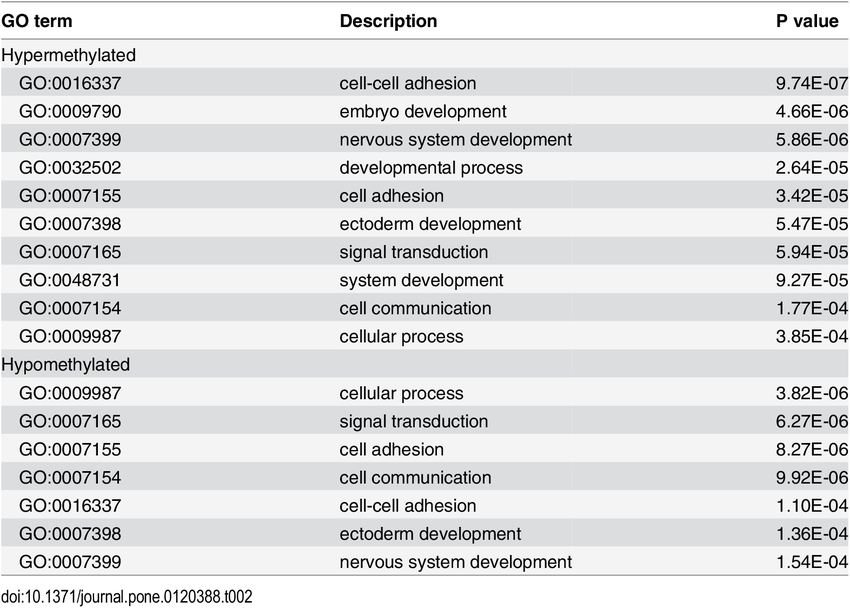
\includegraphics[width=100mm,height=70mm ]{Figures/sample_go.png}
	\caption{Sample GO}
	\label{fig: GO}
\end{figure}

\textit{p-value} here tells us the probability of seeing at least $x$ number of genes out of the total $n$ genes in the list annotated to a particular GO term, given the proportion of genes in the whole genome that are annotated to that GO term. That is, the GO terms shared by the genes in the user's list are compared to the background distribution of annotation. The smaller the \textit{p-value} is, the more significant the particular GO term associated with the group of genes is (i.e. the less likely the observed annotation of the particular GO term to a group of genes occurs by chance).  In other words, when searching the process ontology, if all of the genes in a group were associated with "DNA repair", this term would be significant.

%----------------------------------------------------------------------------------------